\chapter{Applications to $WW$ scattering}
\label{chap:ww}
We now turn to the process $W^+ W^- \to W^+ W^-$. Our goal is to derive positivity constraints on departures from the Standard Model under different assumptions about the number of subtractions required in the dispersion relation.

We begin by studying a phenomenological deformation of the Standard Model in which the masses and couplings entering the scattering amplitudes are treated as independent parameters, rather than being fixed by electroweak symmetry breaking and gauge invariance. From an effective field theory perspective, such deformations can be understood as the low-energy manifestation of higher-dimensional operators. By analysing the positivity bounds under different assumptions about the ultraviolet behaviour of the amplitude, we will obtain constraints on these effective parameters.
We will then extend the analysis by explicitly including dimension-six beyond-the-Standard-Model (BSM) operators and study how the positivity constraints are modified in their presence.

For simplicity, we consider the amplitudes in the limit $\sin\theta_{EW}=0$. In this regime, the electroweak gauge bosons satisfy $m_Z = m_W$, and the trilinear and quartic gauge couplings become equal, $g_Z = g_W$. We will relax these assumptions and explore the effects of allowing $m_Z$ and $g_Z$ to differ from their Standard Model values.

\section{Deformations of the Standard Model}

First, we assume that the scattering amplitude satisfies $0$-th substracted dispersion relations. This requirement is equivalent to demanding that the amplitude vanishes in the high-energy limit, \( s \to \infty \).

Under this assumption, the relevant arc coefficients are:
\begin{align}
    a_0^{(00)} &= -6 g_Z^2 + g_W^2 \left[ 5 + g_h^2 \left( 2 - \frac{m_h^2}{m^2} \right) \right] 
    + \frac{g_Z^2}{m^4 m_Z^2} \left(-4m^6 - 2m^2 m_Z^4 + m_Z^6 \right), \\
    a_1^{(00)} &= 0, \\
    a_2^{(00)} &= \frac{-g_W^2 + g_Z^2}{m^4}, \\
    a_0^{(++)} &= 2g_W^2 - \frac{g_Z^2 (2m^2 + m_Z^2)}{m_Z^2}, \\
    a_1^{(++)} &= - \frac{g_Z^2}{m_Z^2}, \\
    a_2^{(++)} &= 0.
\end{align}

From the positivity of the twice-subtracted arc, \( a_2^{(00)} \geq 0 \), one obtains
\[
\frac{g_Z^2}{g_W^2} \geq 1,
\]
which provides a lower bound on the coupling of the \( Z \) boson to the \( W \) boson.

Combining this with the positivity of the 0-th substracted arc, \( a_0^{(++)} \geq 0 \), yields
\[
m_Z^2 \geq 2 m^2.
\]
This bound already excludes the Standard Model configuration, where \( m_Z^2 = m^2 \).
To complete the analysis, we use the relation between once- and 0-th substracted arcs,
\[
\left| a_1^{(++)} \right| (\Lambda^2 - 2m^2) \leq a_0^{(++)}.
\]
This inequality leads to two distinct regimes:
\begin{equation}
    \begin{cases}
        \dfrac{g_Z^2}{g_W^2} \leq 2 
        \;\Rightarrow\;
        \dfrac{m_Z^2}{\Lambda^2} \geq \dfrac{ \frac{g_Z^2}{g_W^2} }{2 - \frac{g_Z^2}{g_W^2}}, \\[1em]
        \dfrac{g_Z^2}{g_W^2} \geq 2 
        \;\Rightarrow\;
        \dfrac{m_Z^2}{\Lambda^2} \leq \dfrac{ \frac{g_Z^2}{g_W^2} }{2 - \frac{g_Z^2}{g_W^2}} < 0
    \end{cases}
    \label{eq:casesint}
\end{equation}
The second regime, \( g_Z^2 \geq 2 g_W^2 \), is clearly inconsistent. In the first regime, \( g_Z^2 \leq 2 g_W^2 \), there appears to be a viable window. However, combining this with the bound \( g_Z^2 \geq g_W^2 \) implies
\[
m_Z^2 \geq \Lambda^2,
\]
this is the \( Z \)-boson resonance would lie above the cutoff. This is problematic, as the effective theory cannot reliably describe physics above \( \Lambda \). This is summarized in \Cref*{fig:boundsintersction}.
\begin{figure}[hbtp]
    \begin{center}
        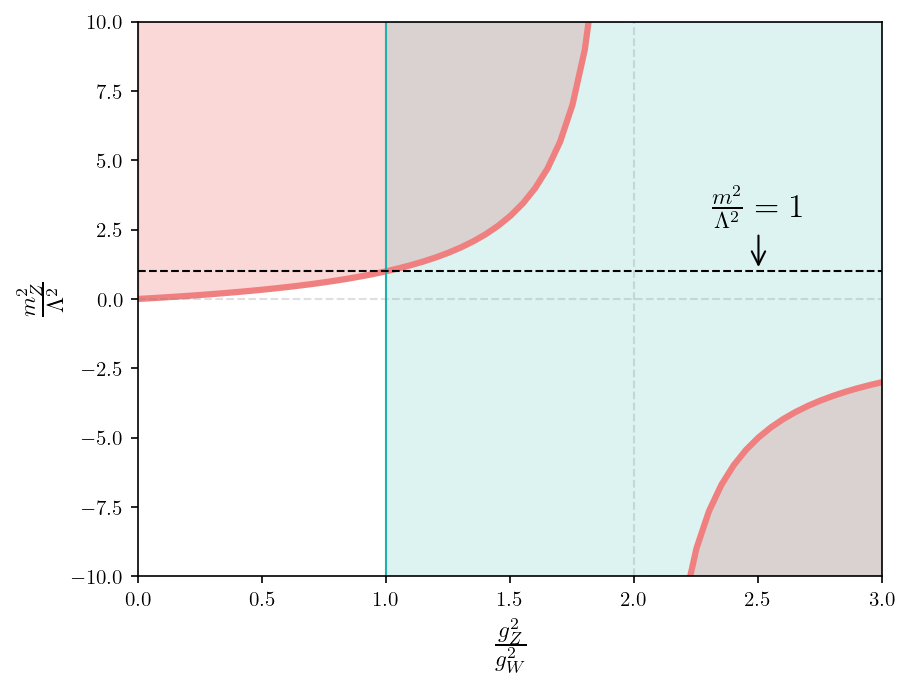
\includegraphics[width= 0.85 \textwidth]{../figures/bounds_intersection.png}
    \end{center}
    \label{fig:boundsintersction}
    \caption{Intersection of the different bounds that appear when assuming the $WW$ scattering fulfils 0-th substracted dispersion relations. The regions highlighted in red correspond to the bounds arising from \Cref*{eq:casesint}, while the region highlighted in blue corresponds to $g_Z^2 \geq g_W^2$.}
\end{figure}

Therefore, the process under consideration is not consistent with unsubtracted dispersion relations. However, it remains compatible with twice-subtracted dispersion relations, provided that \( g_Z^2 \geq g_W^2 \).
This condition is reminiscent of the role of the three-point coupling in ensuring the cancellation of the \( s^2 \) growth in the scattering amplitude for \( W^+_L W^-_L \rightarrow W^+_L W^-_L \). 

\section{Higher-Order Operators}

We now investigate how these bounds are modified in the presence of dimension-six operators. To this end, we fix both the $ZW^+W^-$ and Higgs--$W$ couplings to their Standard Model values, as well as the mass of the $Z$ boson. 
We will consider the only three dimension 6 operators that affect $WW$ scattering, which will enter the amplitudes through the coefficients $c_H, c_{HW}$ and $c_{3W} $.

In this setup, the relevant arcs in the forward limit take the form
\begin{align}
    a_0^{(++)} &= \frac{g_W^2}{m_Z^2} \Big( -1 + 2 (c_{HW} + c_W) m^2 \Big) (2 m^2 - m_Z^2), \\
    a_1^{(++)} &= \frac{g_W^2}{m_Z^2} \Big( -1 + 2 (c_{HW} + c_W) m^2 \Big),\\
    a_2^{(++)} &= 0, \\
    a_0^{(+0)} &= -4g_W^2 \Big( -1 + 2 c_{HW} m^2 + c_W (-2 + 4m^2) \Big).
\end{align}

Imposing the positivity condition
\[
|a_1^{(++)}|(\Lambda^2 - 2m^2) \leq a_0^{(++)},
\]
leads to two possible cases:
\[
\begin{cases}
    -1 + 2 (c_{HW} + c_W)m^2 < 0
    &\Rightarrow\quad m_Z^2 \geq \Lambda^2, \\[4pt]
    -1 + 2 (c_{HW} + c_W)m^2 > 0
    &\Rightarrow\quad m_Z^2 \leq 0.
\end{cases}
\]

Both conditions are physically inconsistent. Therefore, the scattering amplitude remains incompatible with the existence of a 0-th subtracted dispersion relation, even after including dimension-six operators.

The only remaining possibility corresponds to the degenerate case
\[
-1 + 2 (c_{HW} + c_W)m^2 = 0.
\]

In this regime, the condition $a_0^{(+0)} \geq 0$ implies that the physically allowed region with $m^2 \leq \Lambda^2$ exists only for
\[
c_W \geq 0.
\]
Then, no bounds arise whenever
\begin{equation}
\begin{cases}
    c_{HW} + c_W = \dfrac{1}{2m^2}, \\[6pt]
    c_W \geq 0.
\end{cases}
\label{eq:dim6cond}
\end{equation}

The corresponding region in the $(c_W,c_{HW})$ plane is shown in \Cref*{fig:dim6line}.

\begin{figure}[hbtp]
    \begin{center}
        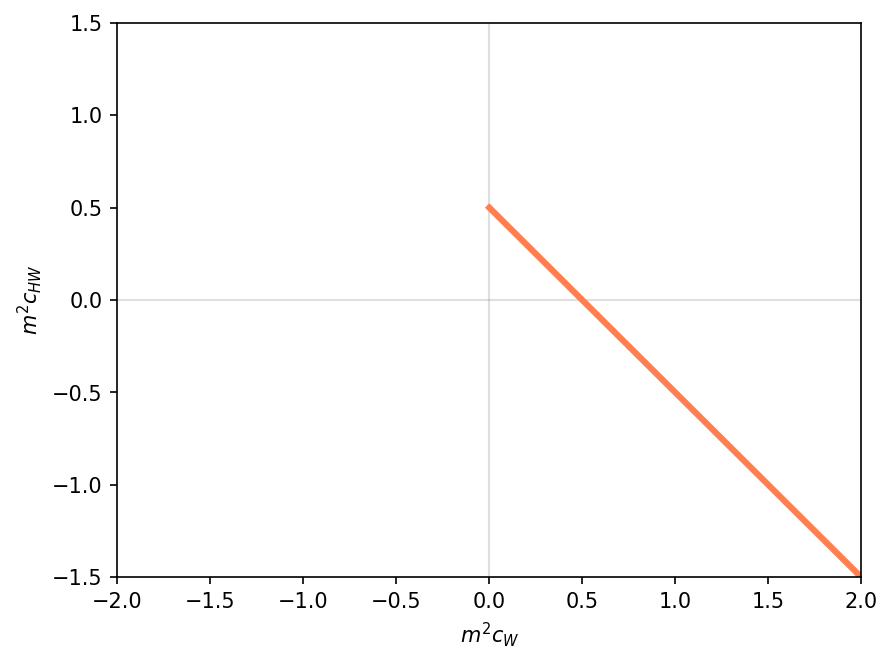
\includegraphics[width=0.75\textwidth]{../figures/dim6.png}
    \end{center}
    \caption{Region in the $(c_W,c_{HW})$ parameter space for which there are no bounds in the spectrum.}
    \label{fig:dim6line}
\end{figure}

\subsection{Finite \texorpdfstring{$t$}{t}}
We now examine whether the fine-tuned regime remains consistent for finite values of $t$.

Up to first order in $t$, the $++$ arc at zero substractions is given by
\begin{equation}
    \begin{aligned}
    a_0^{(++)} = \frac{g_W^2}{m_Z^2} \Big[
    & \big(-1 + 2 (c_{HW} + c_W)m^2\big)(2m^2 - m_Z^2) \\
    & + \big(1 - 2 (c_{HW} + c_W)m^2 + 4 c_{3W} m_Z^2\big)\, t
    \Big].
    \end{aligned}
\end{equation}
In order for this regime to be compatible with \Cref{eq:trumpets}, we must therefore require either $c_{3W} = 0$ or $m_Z = 0$.

We first analyze the case $c_{3W} = 0$. In this regime,
\begin{equation}
m_0^{(+0)} = \frac{2 \Lambda^2 - 3 m^2}{8 m^2 \left(m^2 - \Lambda^2\right)},
\end{equation}
which, as discussed in \Cref{sec:forwardlimit}, must satisfy
\begin{equation}
-\frac{1}{2(\Lambda^2 - 2m^2)}
\leq
m_0^{(+0)}
\leq
\frac{1}{2 \Lambda^2 - 4 m^2 + t} - \frac{2}{t}.
\end{equation}

We focus on the lower bound, since it is independent of $t$. Rewriting the constraint yields
\begin{equation}
\frac{2 \Lambda^2 - 3 m^2}{8 m^2 (m^2 - \Lambda^2)}
- \frac{1}{2(\Lambda^2 - 2m^2)}
\geq 0,
\end{equation}
which is satisfied only if
\begin{equation}
\frac{m^2}{\Lambda^2} \geq 0.229844.
\end{equation}

We therefore conclude that, if $c_{3W} = 0$, one cannot reach the limit $m = 0$.

We can repeat this analysis for $c_{3W} \neq 0$.
For longitudinal polarizations, using the relation between $c_W$ and $c_{HW}$ and imposing that $m_Z = 0$, we obtain
\begin{equation}
m_0^{(00)} =
\frac{-1 + (c_H - 8 c_W)m^2 - c_W m_h^2}
{2\left[-1 + (c_H - 2c_W)m^2\right](2m^2 - m_h^2)}.
\end{equation}
Note that there are no contributions of $m_Z$. This is a consequence of the condition in \Cref*{eq:dim6cond}, which cancels those terms.

Positivity requires this quantity to satisfy
\begin{equation}
    -\frac{1}{2(\Lambda^2-2m^2)}
    \leq
    m_0^{(00)}
    \leq
    \frac{1}{2 \Lambda^2-4 m^2+t}-\frac{2}{t} .
\end{equation}

We determine numerically the regions of parameter space compatible with these bounds. The resulting allowed regions are displayed in \Cref{fig:many6dim}.
\begin{figure}[hbtp]
    \centering
    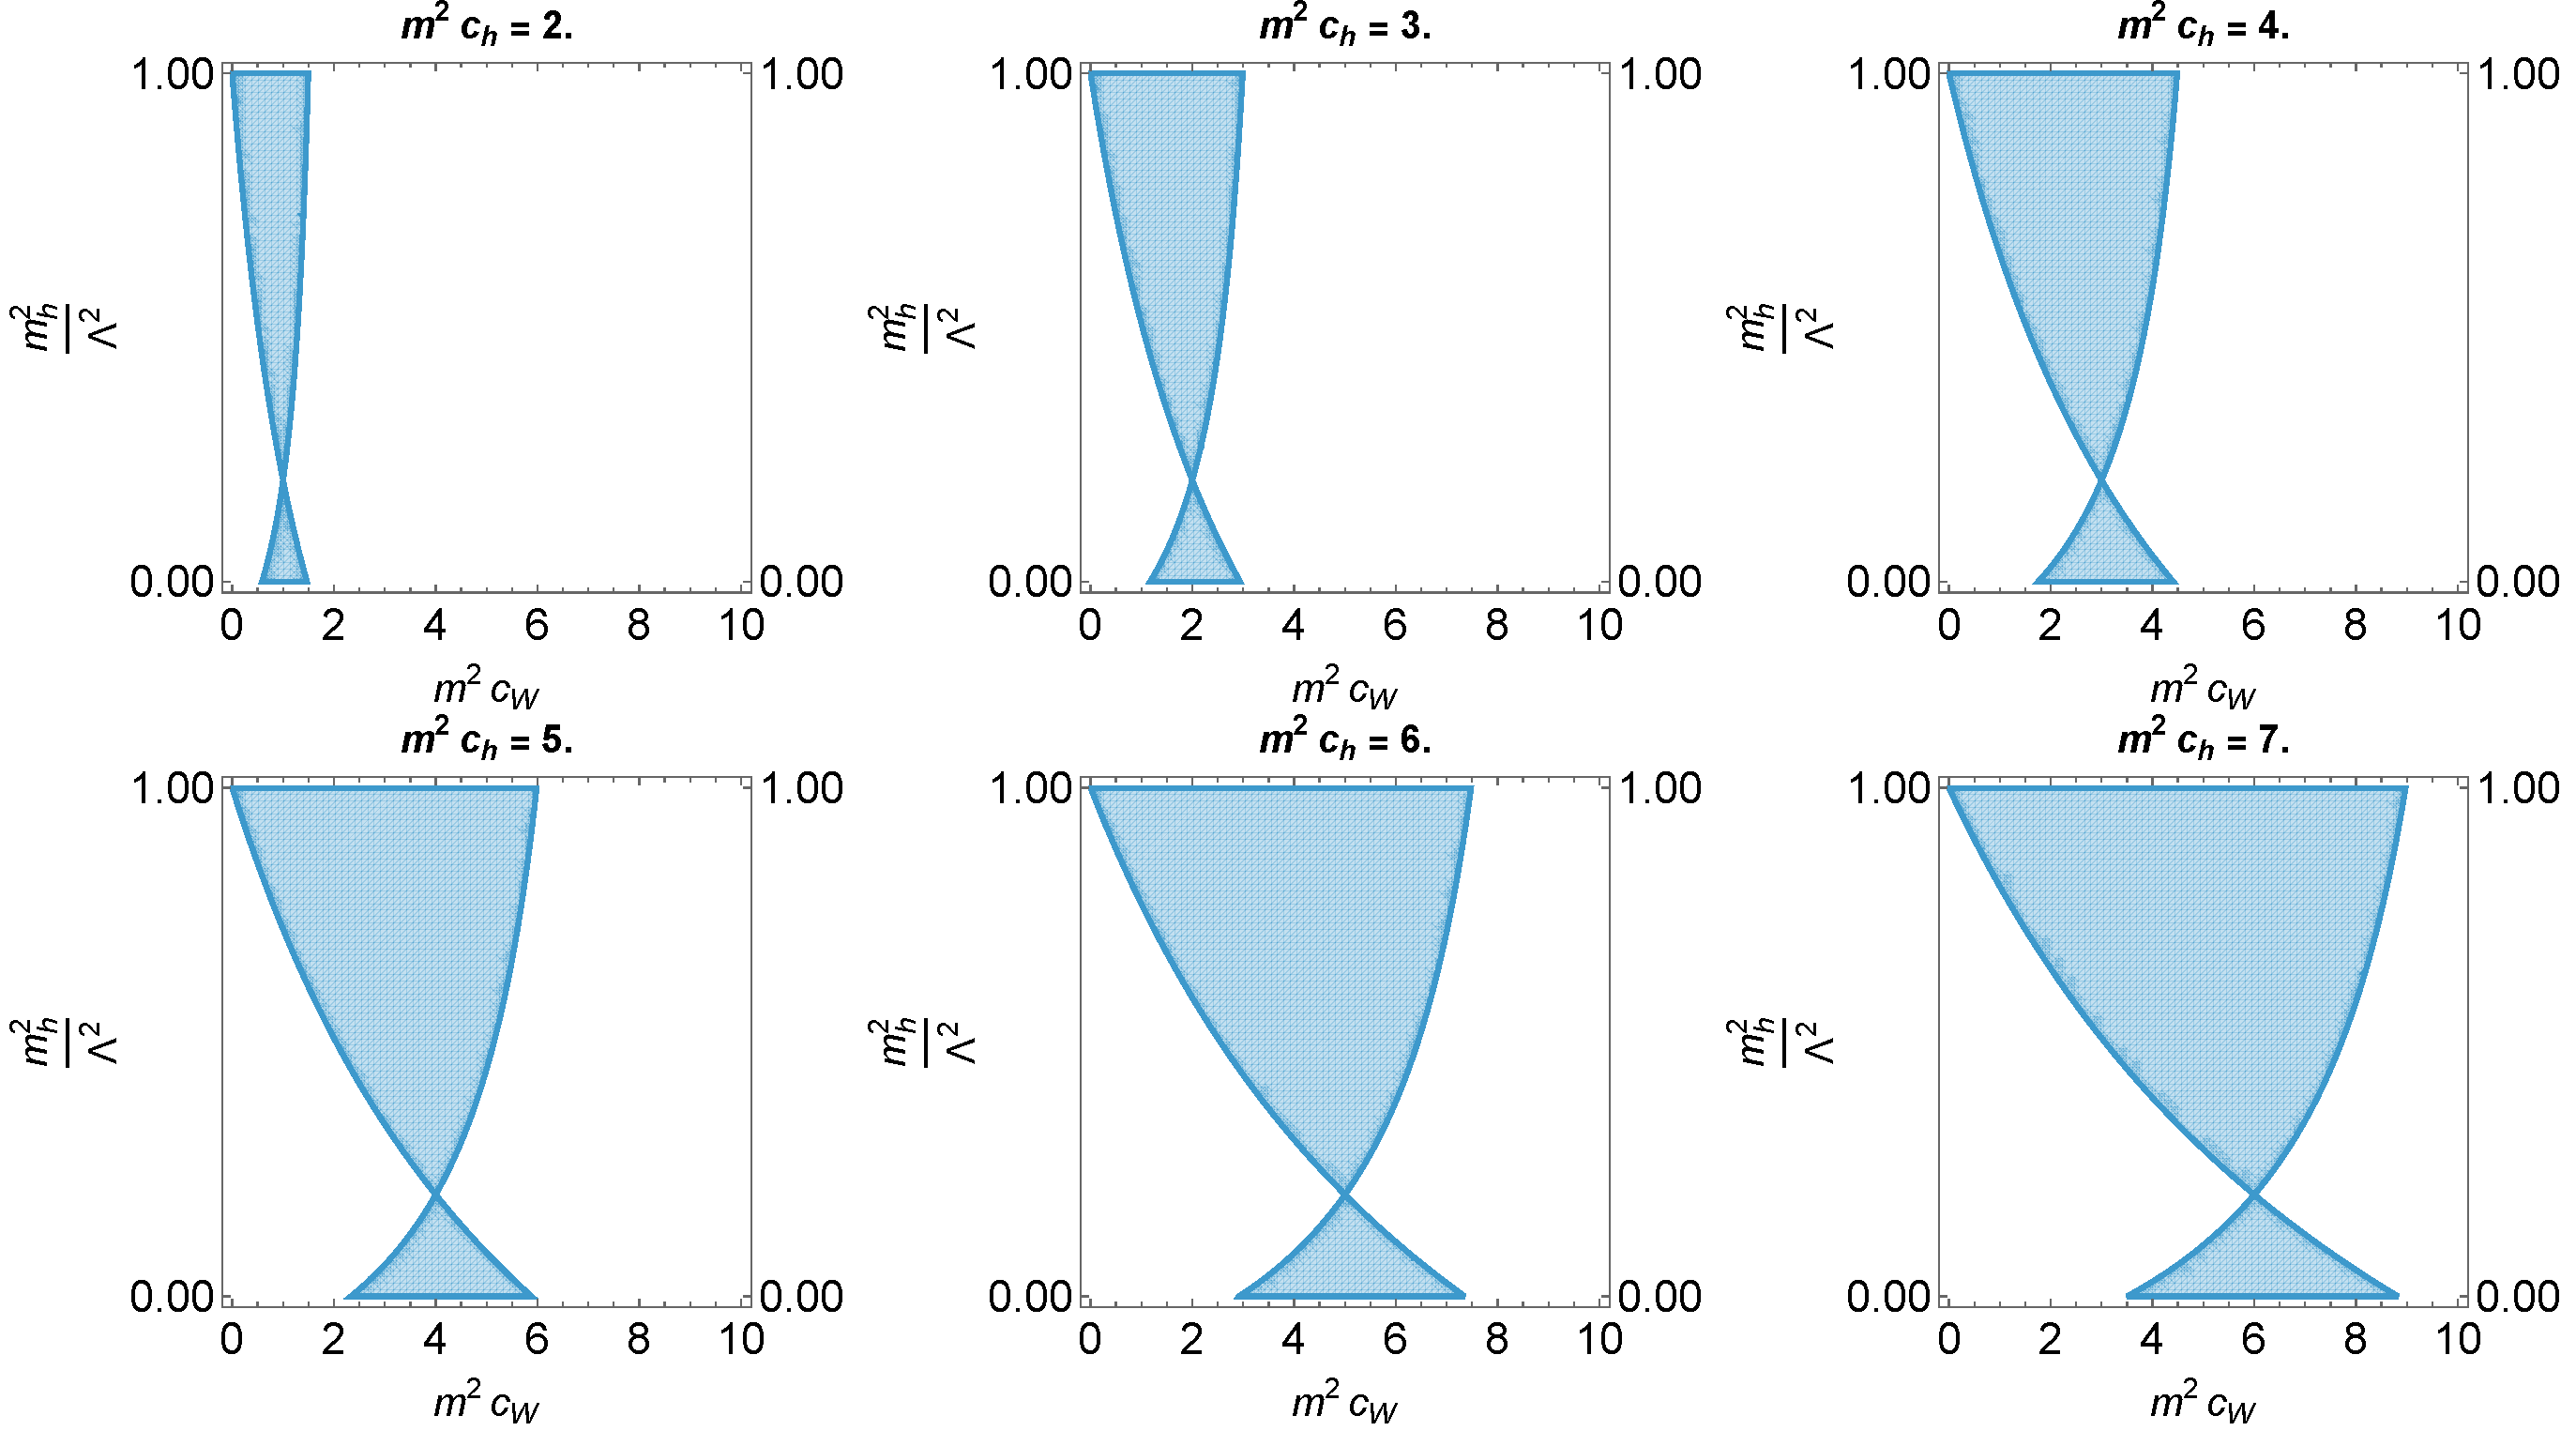
\includegraphics[width=\textwidth]{../figures/dim6_finitet.pdf}
    \caption{Regions of parameter space compatible with the positivity bounds for $t =- 0.1\,\Lambda^2$, including dimension 4 and dimension 6 operators and assuming that $c_{HW} + c_{W} = 1/(2m^2)$ and $c_W \geq 0$.}
    \label{fig:many6dim}
\end{figure}

Several features emerge from the numerical analysis. Most notably, the positivity constraints strongly restrict the relative size of the Wilson coefficients. In particular, we observe that the allowed values of $c_W$ cannot become parametrically larger than those of $c_H$. 

We find no bounds if the amplitude only verifies twice substracted dispersion relations.

\section{Odd Number of Subtractions}
So far, we have derived bounds for $WW$ scattering under the assumption that the amplitude satisfies unsubtracted dispersion relations. It is also interesting to investigate the bounds that arise when the amplitude instead satisfies once-subtracted dispersion relations. However, as discussed in \Cref*{sec:nopos}, no positive sum rules exist for amplitudes with an even number of subtractions.

There is still a way to circumvent this limitation: one can assume that the crossed amplitude appearing in the dispersive integral is analytic. In that case, the crossed channel does not contribute to the sum rules, making it possible to obtain positivity bounds even in the presence of an odd number of subtractions.

In this section, we consider fixed-$u$ dispersion relations. The crossed process is then $W^+ W^+ \to W^+ W^+$, corresponding to the isospin-$2$ amplitude. Assuming analyticity for this channel is equivalent to treating the $W$ bosons as composite states made of isospin-$1/2$ constituents in the large-$N$ limit \autocite{Albert:2022oes}.

\subsection{Deformations of the Standard Model}
Keeping only the Standard Model operators, the relevant arcs in the $u \to 0$ limit are 
\begin{align}
    a_1^{(00)} &= 4  \left( \frac{g_Z^2 - g_W^2}{m^2} + \frac{g_Z^2 }{m_Z^2} \right), \\
    a_2^{(00)} &= \frac{g_Z^2 - g_W^2}{2m^4}.
\end{align}
From $a_2^{(00)} \geq 0$, we recover the condition that $g_Z \geq 1$. Using the relation $a_2 (\Lambda^2 - 2m^2) \leq a_1$, we find the upper bounds for $g_Z$ shown in figure \Cref*{fig:nomz}.
\begin{figure}[hbtp]
    \begin{center}
        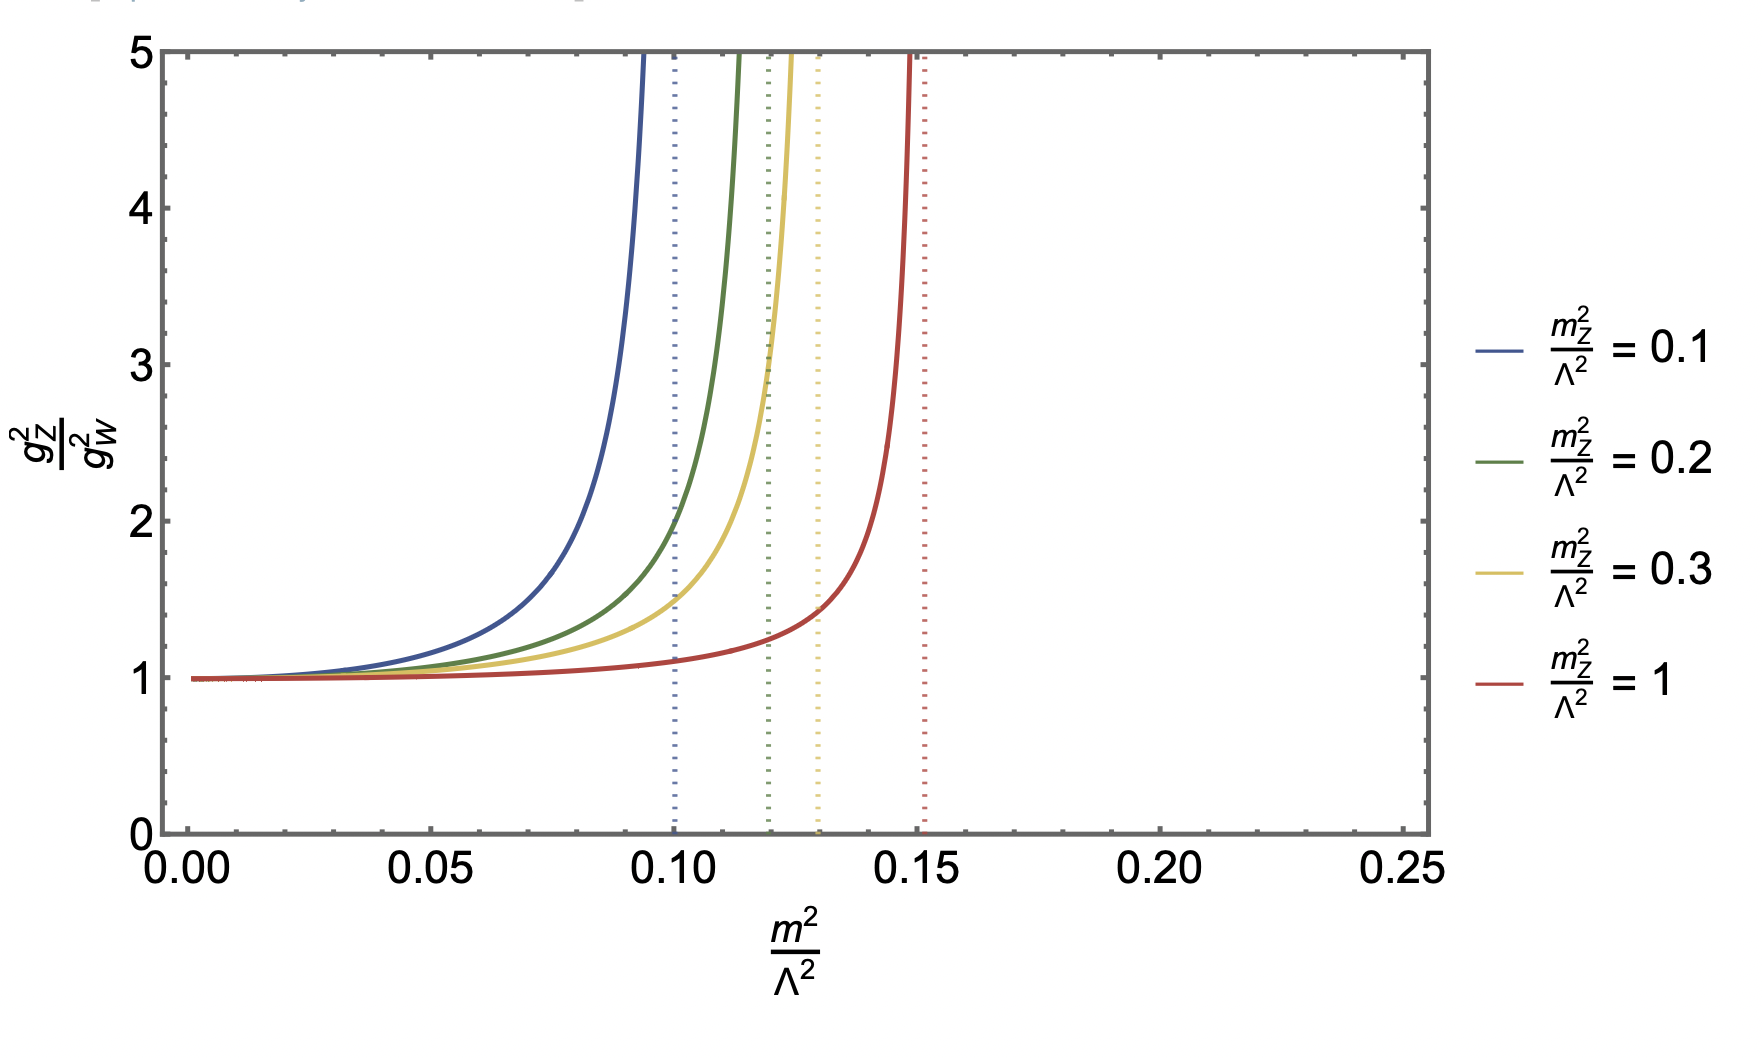
\includegraphics[width = 0.85 \textwidth]{../figures/1sub_nomZ.png}
    \end{center}
    \caption{Upper bound in $g_Z$ for different values of $m^2$ and $m_Z^2$, only including dimension 4 operators and assuming the isospin-2 amplitude is analytical. The dashed lines represent the value of $m^2$ starting from which the theory is not consistent, as it gives $g_Z < 0$.}
    \label{fig:nomz}
\end{figure}
As we can see, taking the cutoff to the infinity implies that $g_Z = 1$, which brings us back to the Standard Model.

It is also interesting to study the $m_Z^2 = m^2$ case. For this, the allowed region for $m^2$ is shown in \Cref*{fig:withmz}. The cutoff can not be taken to $\infty$ unless we choose the Standard Model coupling, $g_Z$. If $m^2/ \Lambda^2 \geq 1/10$, the setup is consistent for any value of $g_Z$. Adding information from the first order in $u$ does not improve these bounds.
\begin{figure}[hbtp]
    \begin{center}
        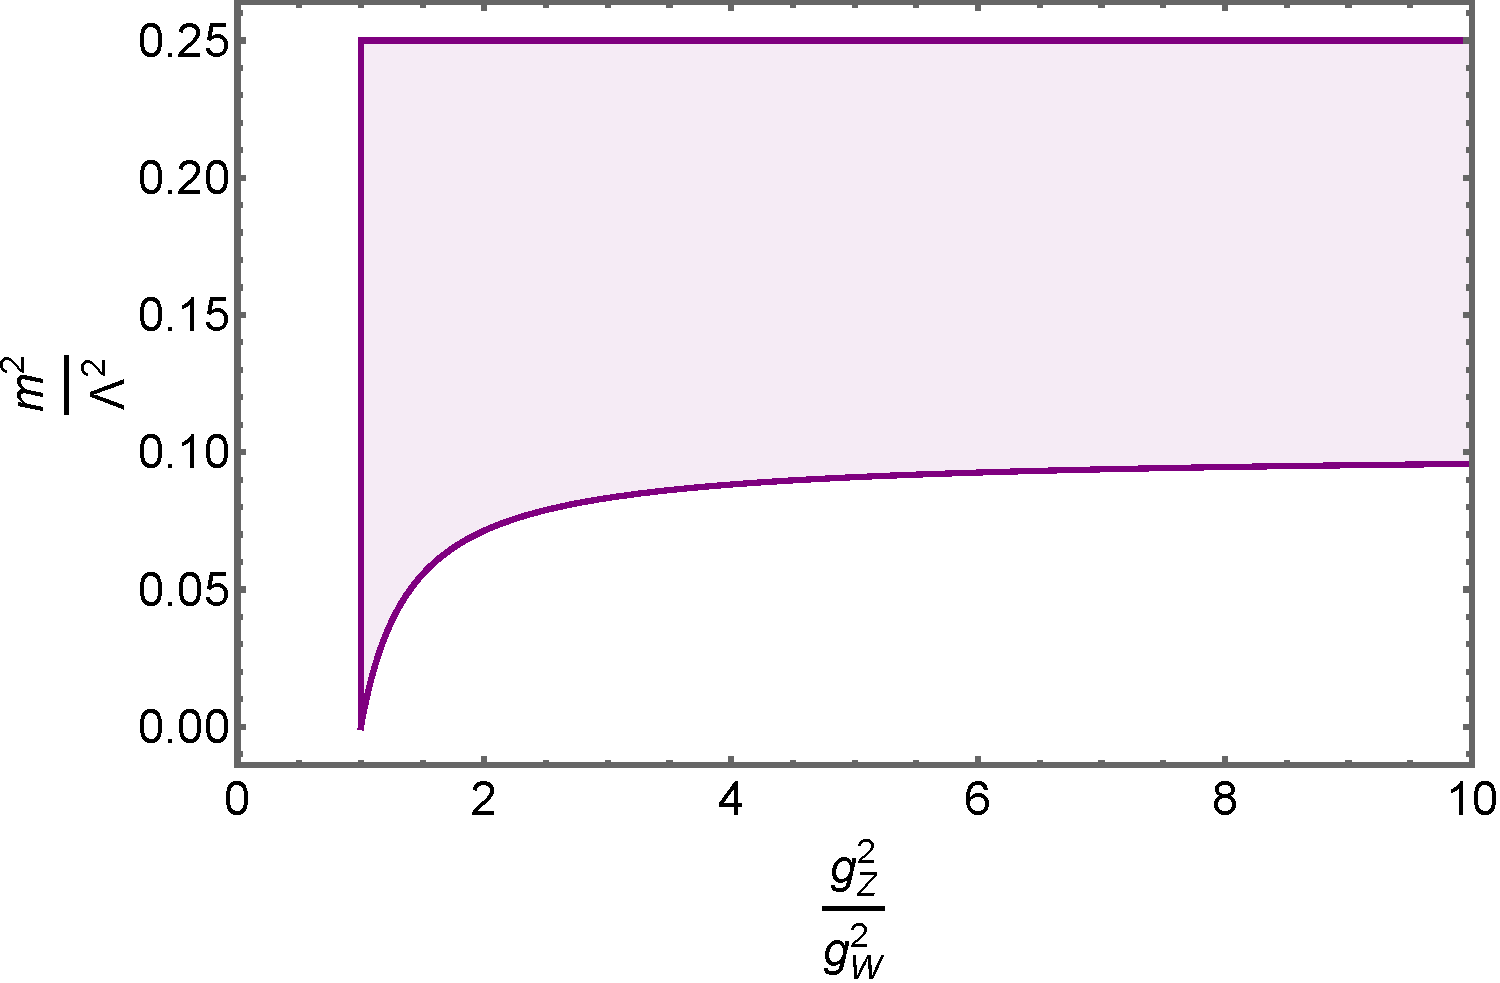
\includegraphics[width = 0.85 \textwidth]{../figures/image.pdf}
    \end{center}
    \caption{Allowed region for $m^2$ for differentes values in $g_Z$, only including dimension 4 operators and assuming the isospin-2 amplitude is analytical.}
    \label{fig:withmz}
\end{figure}
\subsection{Higher-Order Operators}
Lastly, we study how these bounds are modified by the inclusion of dimension-6 operators. Restricting again to the regime $m^2 = m_Z^2$, the relevant arcs, up to first order in $u$, are
\begin{equation}
    a_1^{(00)}(u) = -g_W^2\frac{ 16 m^4 (c_{HW}+c_{W})-4 m^2 \left(3 c_W m_Z^2+2\right)+c_W
    m_Z^2 \left(4 m_h^2+u \right) }{2 m^2 m_Z^2}.
\end{equation}
\begin{equation}
    a_2^{(00)}(u) = 0, 
\end{equation}

Using that
\[
0 \leq a_2^{(00)}(\Lambda^2 - 2m^2) \leq a_1^{(00)},
\]
and imposing boundedness of the contribution linear in $u$, we numerically solve the resulting system of inequalities to derive constraints on $m^2$ and $m_h^2$.

We find that, once dimension-6 operators are included, no absolute bounds on the spectrum can be obtained independently of the higher-order operators. Nevertheless, as shown in \Cref{fig:space_no_branch_cut}, positivity still imposes non-trivial restrictions on the allowed parameter space for different choices of the $W$ and Higgs boson masses.

\begin{figure}[hbtp]
    \begin{center}
        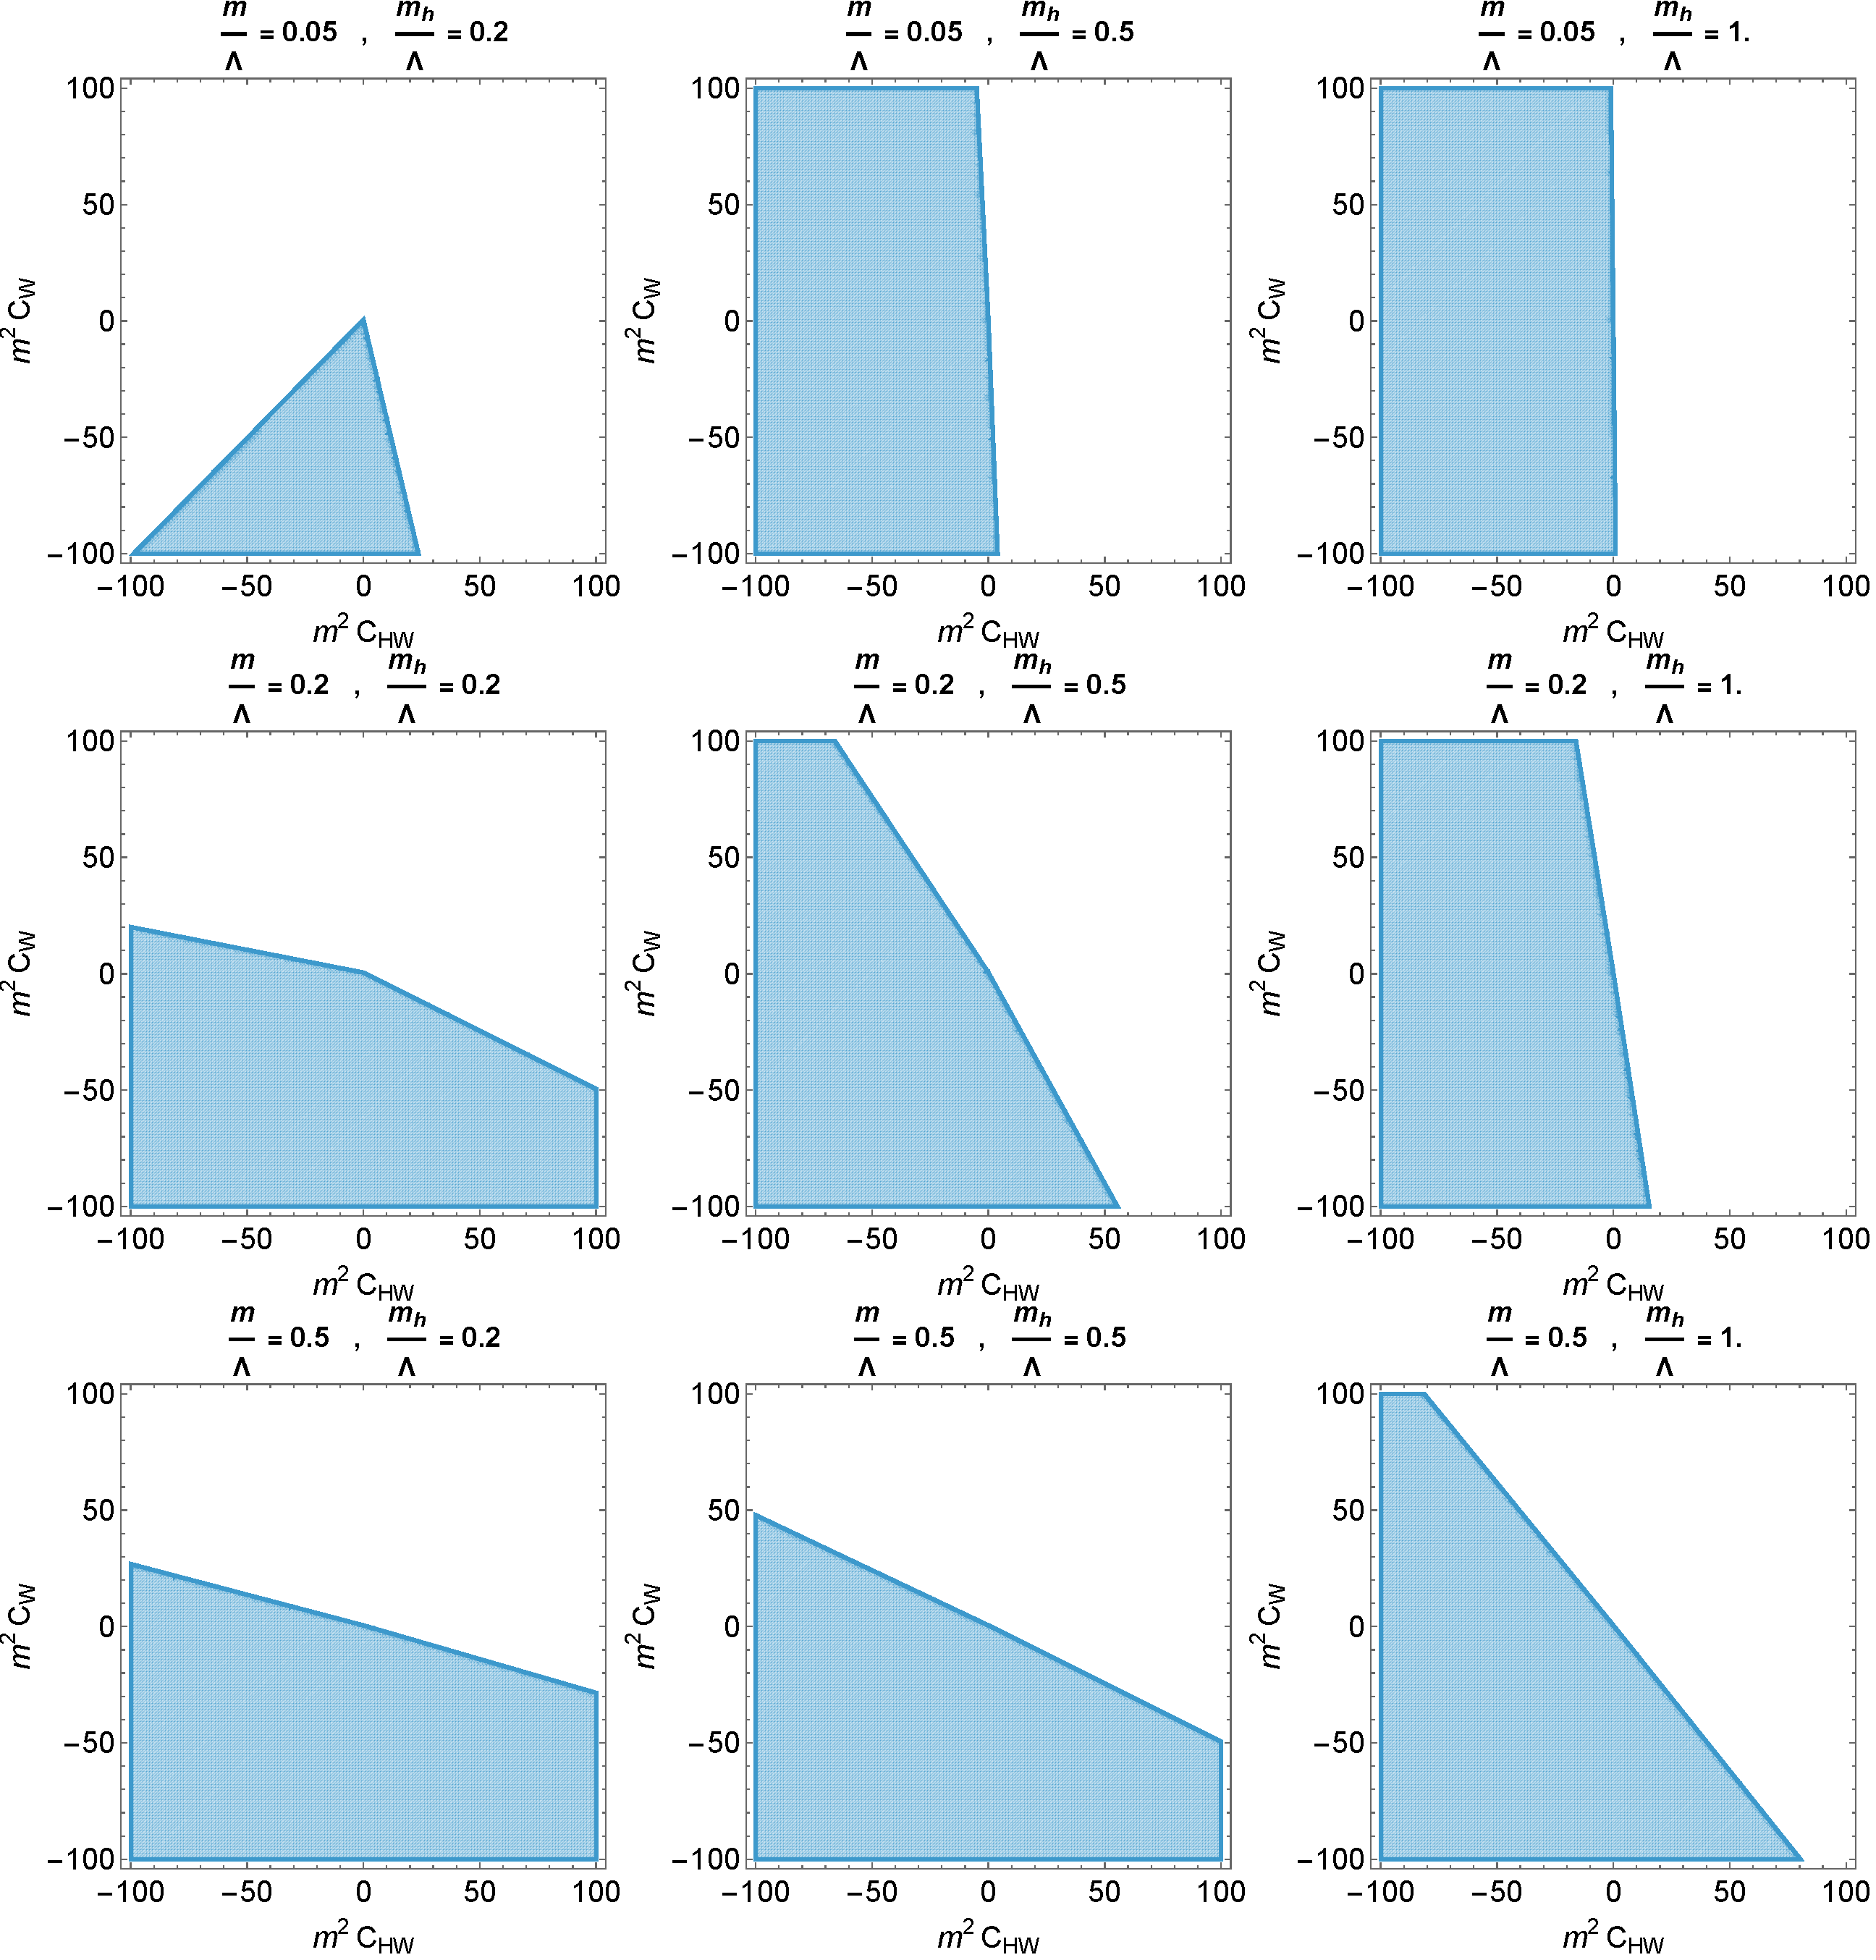
\includegraphics[width=\textwidth]{../figures/no_branch_cut_space.pdf}
    \end{center}
    \caption{Regions of parameter space compatible with the positivity bounds for different values of $m$ and $m_h$, for $u=-0.1\Lambda^2$, assuming once-subtracted dispersion relations and analyticity of the isospin-2 channel.}
    \label{fig:space_no_branch_cut}
\end{figure}
